\documentclass{beamer}
\usepackage{lipsum}
\usepackage{tikz}
\usepackage{shellesc}
\usepackage{pdftexcmds}
\usepackage{robust-externalize}
\usetikzlibrary{positioning, decorations.pathreplacing, calc, arrows.meta, shapes.geometric, backgrounds}
\robExtConfigure{enable fallback to manual mode} % prints command to run in PDF if shell-escape is not used/forgotten
\def\mathdefault#1{#1} % Needed in matplotlib 3.8: https://github.com/matplotlib/matplotlib/issues/27907
\setbeamertemplate{frametitle}[default][center]

\tikzset{
    bigbox/.style={draw, rounded corners, minimum width=1.5cm, minimum height=1cm},
    smallbox/.style={draw, rounded corners, minimum width=1.25cm, minimum height=0.75cm},
    bigcircle/.style={draw, circle, minimum size=1cm},
    bigellipse/.style={draw, ellipse, minimum width=1.5cm, minimum height=1.25cm},
    place/.style={inner sep=0pt, outer sep=0pt},
    fork/.style={decorate, decoration={show path construction, lineto code={
        \draw[->](\tikzinputsegmentfirst)-|($(\tikzinputsegmentfirst)!.5!(\tikzinputsegmentlast)$)|-(\tikzinputsegmentlast);}
    }},
    center coordinate/.style={
        execute at end picture={
        \path ([rotate around={180:#1}]perpendicular cs: horizontal line through={#1},
                                    vertical line through={(current bounding box.east)})
                ([rotate around={180:#1}]perpendicular cs: horizontal line through={#1},
                                    vertical line through={(current bounding box.west)});}}
}


\title{Sample title}
\author{Anonymous}
\institute{Overleaf}
\date{2021}

\begin{document}

\frame{\titlepage}

\begin{frame}[fragile]
\frametitle{Seed and Extend approach}

{\centering
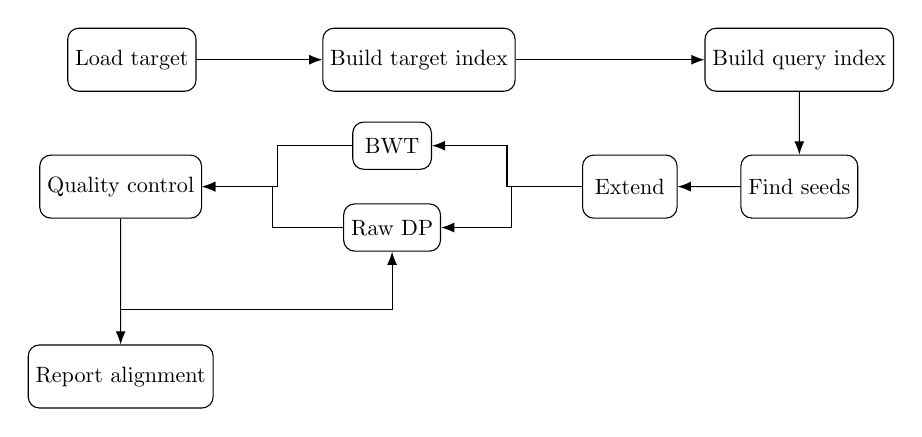
\begin{tikzpicture}[scale=.8, transform shape, node distance=1cm, >=Latex]
  \node(LT)[bigbox]{Load target};
  \node(TI)[bigbox, right=2cm of LT]{Build target index};
  \node(LQ)[bigbox, right=3cm of TI]{Build query index};
  \node(S)[bigbox, below=of LQ]{Find seeds};
  \node(E)[bigbox, left=of S]{Extend};


  \node[place](X)[left=3cm of E]{};
  \node(ABWT)[smallbox, above=2.5mm of X]{BWT};
  \node(ADP)[smallbox, below=2.5mm of X]{Raw DP};

  \node(QC)[bigbox, left=3cm of X]{Quality control};
  \node(R)[bigbox, below=2cm of QC]{Report alignment};

  \draw[->](LT)--(TI);
  \draw[->](TI)--(LQ);
  \draw[->](LQ)--(S);
  \draw[->](S)--(E);
  \draw[->](QC)--(R);

  \draw[fork](E.west)--(ABWT.east);
  \draw[fork](E.west)--(ADP.east);

  \draw[fork](ABWT.west)--(QC.east);
  \draw[fork](ADP.west)--(QC.east);

  %\draw[fork](QC.south)--(ADP.south);

  \path ($(R)!0.45!(ADP)$) -| (QC) coordinate [pos=0.2] (aux);
  \draw (QC) |- (aux);
  \draw[->] (aux) -| (ADP);

\end{tikzpicture}
\par}

\end{frame}

\begin{frame}[fragile]
\frametitle{Sample frame title}

\begin{figure}[ht]
  \centering
  \begin{CacheMeCode}{python, custom include command={\input{\robExtAddCachePathAndName{\robExtFinalHash.pgf}}}, set placeholder eval={__LINEWIDTH__}{\lenToCmNoUnit[in]{\linewidth}}}
    import matplotlib.pyplot as plt
    import matplotlib
    import numpy as np
    import json
    matplotlib.use("pgf")
    #### See this link for details on how to preview the image in jupyter
    #### https://matplotlib.org/stable/users/explain/text/pgf.html
    matplotlib.rcParams.update({
      "font.family": "serif",
      "font.serif": [], # Use LaTeX default serif font.
      "text.usetex": True, # use inline math for ticks
      #### You can change the font size of individual items with:
      #### "font.size": 11,
      #### "axes.titlesize": 11,
      #### "legend.fontsize": 11,
      #### "axes.labelsize": 11,
    })
    
    with open('../data1.json') as f:
        stats = json.load(f)
    fig, ax = plt.subplots()
    fig.set_size_inches(__LINEWIDTH__, 0.7*__LINEWIDTH__, forward=True)
    cases = list({case_name for program_label, program_stats in stats.items() for case_name in program_stats})
    width = 0.25
    multiplier = 0
    x = np.arange(len(cases))
    for program_label, program_stats in stats.items():
        offset = width * multiplier
        rects = ax.bar(x + offset, [program_stats[case]["total_execution"]["t_total"] for case in cases], width, label=program_label)
        ax.bar_label(rects, padding=3)
        multiplier += 1

    ax.set_xticks(x + width/2)
    ax.set_xticklabels([case.replace('_', '-') for case in cases])
    ax.set_ylabel('Execution time [ms]')
    ax.set_title("Total execution time")
    ax.legend(title='Program')

    print(get_filename_from_extension(".pgf"))
    plt.savefig(get_filename_from_extension(".pgf"), bbox_inches="tight")
  \end{CacheMeCode}
  \caption{Test}%
\end{figure}

\end{frame}

\begin{frame}[fragile]
  \frametitle{Sample frame title}

  \begin{tikzpicture}[
    scale=5,
    axis/.style={very thick, ->, >=stealth'},
    important line/.style={thick},
    dashed line/.style={dashed, thin},
    pile/.style={thick, ->, >=stealth', shorten <=2pt, shorten
    >=2pt},
    every node/.style={color=black}
    ]
    % axis
    \draw[axis] (-0.1,0)  -- (1.1,0) node(xline)[right]
        {$G\uparrow/T\downarrow$};
    \draw[axis] (0,-0.1) -- (0,1.1) node(yline)[above] {$E$};
    % Lines
    \draw[important line] (.15,.15) coordinate (A) -- (.85,.85)
        coordinate (B) node[right, text width=5em] {$Y^O$};
    \draw[important line] (.15,.85) coordinate (C) -- (.85,.15)
        coordinate (D) node[right, text width=5em] {$\mathit{NX}=x$};
    % Intersection of lines
    \fill[red] (intersection cs:
       first line={(A) -- (B)},
       second line={(C) -- (D)}) coordinate (E) circle (.4pt)
       node[above,] {$A$};
    % The E point is placed more or less randomly
    \fill[red]  (E) +(-.075cm,-.2cm) coordinate (out) circle (.4pt)
        node[below left] {$B$};
    % Line connecting out and ext balances
    \draw [pile] (out) -- (intersection of A--B and out--[shift={(0:1pt)}]out)
        coordinate (extbal);
    \fill[red] (extbal) circle (.4pt) node[above] {$C$};
    % line connecting  out and int balances
    \draw [pile] (out) -- (intersection of C--D and out--[shift={(0:1pt)}]out)
        coordinate (intbal);
    \fill[red] (intbal) circle (.4pt) node[above] {$D$};
    % line between out og all balanced out :)
    \draw[pile] (out) -- (E);
  \end{tikzpicture}
\end{frame}

\end{document}


% % Local Variables:
% % TeX-command-extra-options: "--shell-escape -halt-on-error"
% % End: